\documentclass[11pt, a4paper]{article}
\usepackage{pdfpages}
\usepackage{parallel}
\usepackage[T2A]{fontenc}
%\usepackage{ucs}
\usepackage[utf8]{inputenc}
\usepackage[english,russian]{babel}
\usepackage{hyperref}
\usepackage{rotating}
\usepackage[inner=2cm,top=1.8cm,outer=2cm,bottom=2.3cm,nohead]{geometry}
%\usepackage{listings}
\usepackage{graphicx}
\usepackage{wrapfig}
\usepackage{longtable}
\usepackage{indentfirst}
\usepackage{array}
\usepackage{tikzsymbols}
\usepackage{soul}
\usepackage[ruled,vlined]{algorithm2e}
\usepackage{qrcode}
\counterwithout{figure}{section} 

\usepackage{url}
\makeatletter
\g@addto@macro{\UrlBreaks}{\UrlOrds}
\makeatother

\newcolumntype{P}[1]{>{\raggedright\arraybackslash}p{#1}}
\frenchspacing
%\usepackage{fixltx2e} %text sub- and superscripts
\usepackage{icomma} % коскі ў матэматычным рэжыме
%\PreloadUnicodePage{4}

\newcommand{\longpage}{\enlargethispage{\baselineskip}}
\newcommand{\shortpage}{\enlargethispage{-\baselineskip}}

\def\switchlang#1{\expandafter\csname switchlang#1\endcsname}
\def\switchlangbe{
\let\saverefname=\refname%
\def\refname{Літаратура}%
\def\figurename{Іл.}%
}
\def\switchlangru{
\let\saverefname=\refname%
\let\savefigurename=\figurename%
\def\refname{Литература}%
\def\figurename{Рис.}%
}
\def\switchlangen{
\let\saverefname=\refname%
\def\refname{References}%
\def\figurename{Fig.}%
}

\hyphenation{admi-ni-stra-tive}
\hyphenation{ex-pe-ri-ence}
\hyphenation{fle-xi-bi-li-ty}
\hyphenation{Py-thon}
\hyphenation{ma-the-ma-ti-cal}
\hyphenation{re-ported}
\hyphenation{imp-le-menta-tions}
\hyphenation{pro-vides}
\hyphenation{en-gi-neering}
\hyphenation{com-pa-ti-bi-li-ty}
\hyphenation{im-pos-sible}
\hyphenation{desk-top}
\hyphenation{elec-tro-nic}
\hyphenation{com-pa-ny}
\hyphenation{de-ve-lop-ment}
\hyphenation{de-ve-loping}
\hyphenation{de-ve-lop}
\hyphenation{da-ta-ba-se}
\hyphenation{plat-forms}
\hyphenation{or-ga-ni-za-tion}
\hyphenation{pro-gramming}
\hyphenation{in-stru-ments}
\hyphenation{Li-nux}
\hyphenation{sour-ce}
\hyphenation{en-vi-ron-ment}
\hyphenation{Te-le-pathy}
\hyphenation{Li-nux-ov-ka}
\hyphenation{Open-BSD}
\hyphenation{Free-BSD}
\hyphenation{men-ti-on-ed}
\hyphenation{app-li-ca-tion}

\def\progref!#1!{\texttt{#1}}
\renewcommand{\arraystretch}{2} %Іначай формулы ў матрыцы зліпаюцца з лініямі
\usepackage{array}

\def\interview #1 (#2), #3, #4, #5\par{

\section[#1, #3, #4]{#1 -- #3, #4}
\def\qname{LVEE}
\def\aname{#1}
\def\q ##1\par{{\noindent \bf \qname: ##1 }\par}
\def\a{{\noindent \bf \aname: } \def\qname{L}\def\aname{#2}}
}

\def\interview* #1 (#2), #3, #4, #5\par{

\section*{#1\\{\small\rm #3, #4. #5}}
\ifx\ParallelWhichBox\undefined%
    \addcontentsline{toc}{section}{#1, #3, #4}%
\else%
\ifnum\ParallelWhichBox=0%
    \addcontentsline{toc}{section}{#1, #3, #4}%
\fi\fi%

\def\qname{LVEE}
\def\aname{#1}
\def\q ##1\par{{\noindent \bf \qname: ##1 }\par}
\def\a{{\noindent \bf \aname: } \def\qname{L}\def\aname{#2}}
}

\newcommand{\interviewfooter}[1]{
\vskip 1em
\noindent \textit{#1}
}

\AtEndDocument{\vfill\centering \qrcode{https://github.com/fiowro/mouses/blob/main/\jobname.pdf}}

\switchlang{en}
\begin{document}

\title{1987 -- Microsoft Dove Bar Mouse}
\date{}
\maketitle
\selectlanguage{english}

The mouse, nicknamed the ``Dove Bar Mouse'' by users because of the similarly shaped soap bar, went on sale in 1987, becoming the third generation of Microsoft mice. The design was developed by Microsoft in collaboration with Matrix Design (which later merged with Hovey-Kelley, the designers of the Apple Lisa mouse, to become the design company IDEO). The mouse's production, as with previous generations of Microsoft mice, was outsourced to the Japanese company Alps. This is probably the first mouse for which the designers set the ergonomics as their main goal. First of all, this resulted in the shape of the body inspired by a sanding block, which automatically ensured a comfortable hand position, worked out on many generations of people \cite{doveBarDesign1, atkinson}.

\begin{figure}[h]
   \centering
    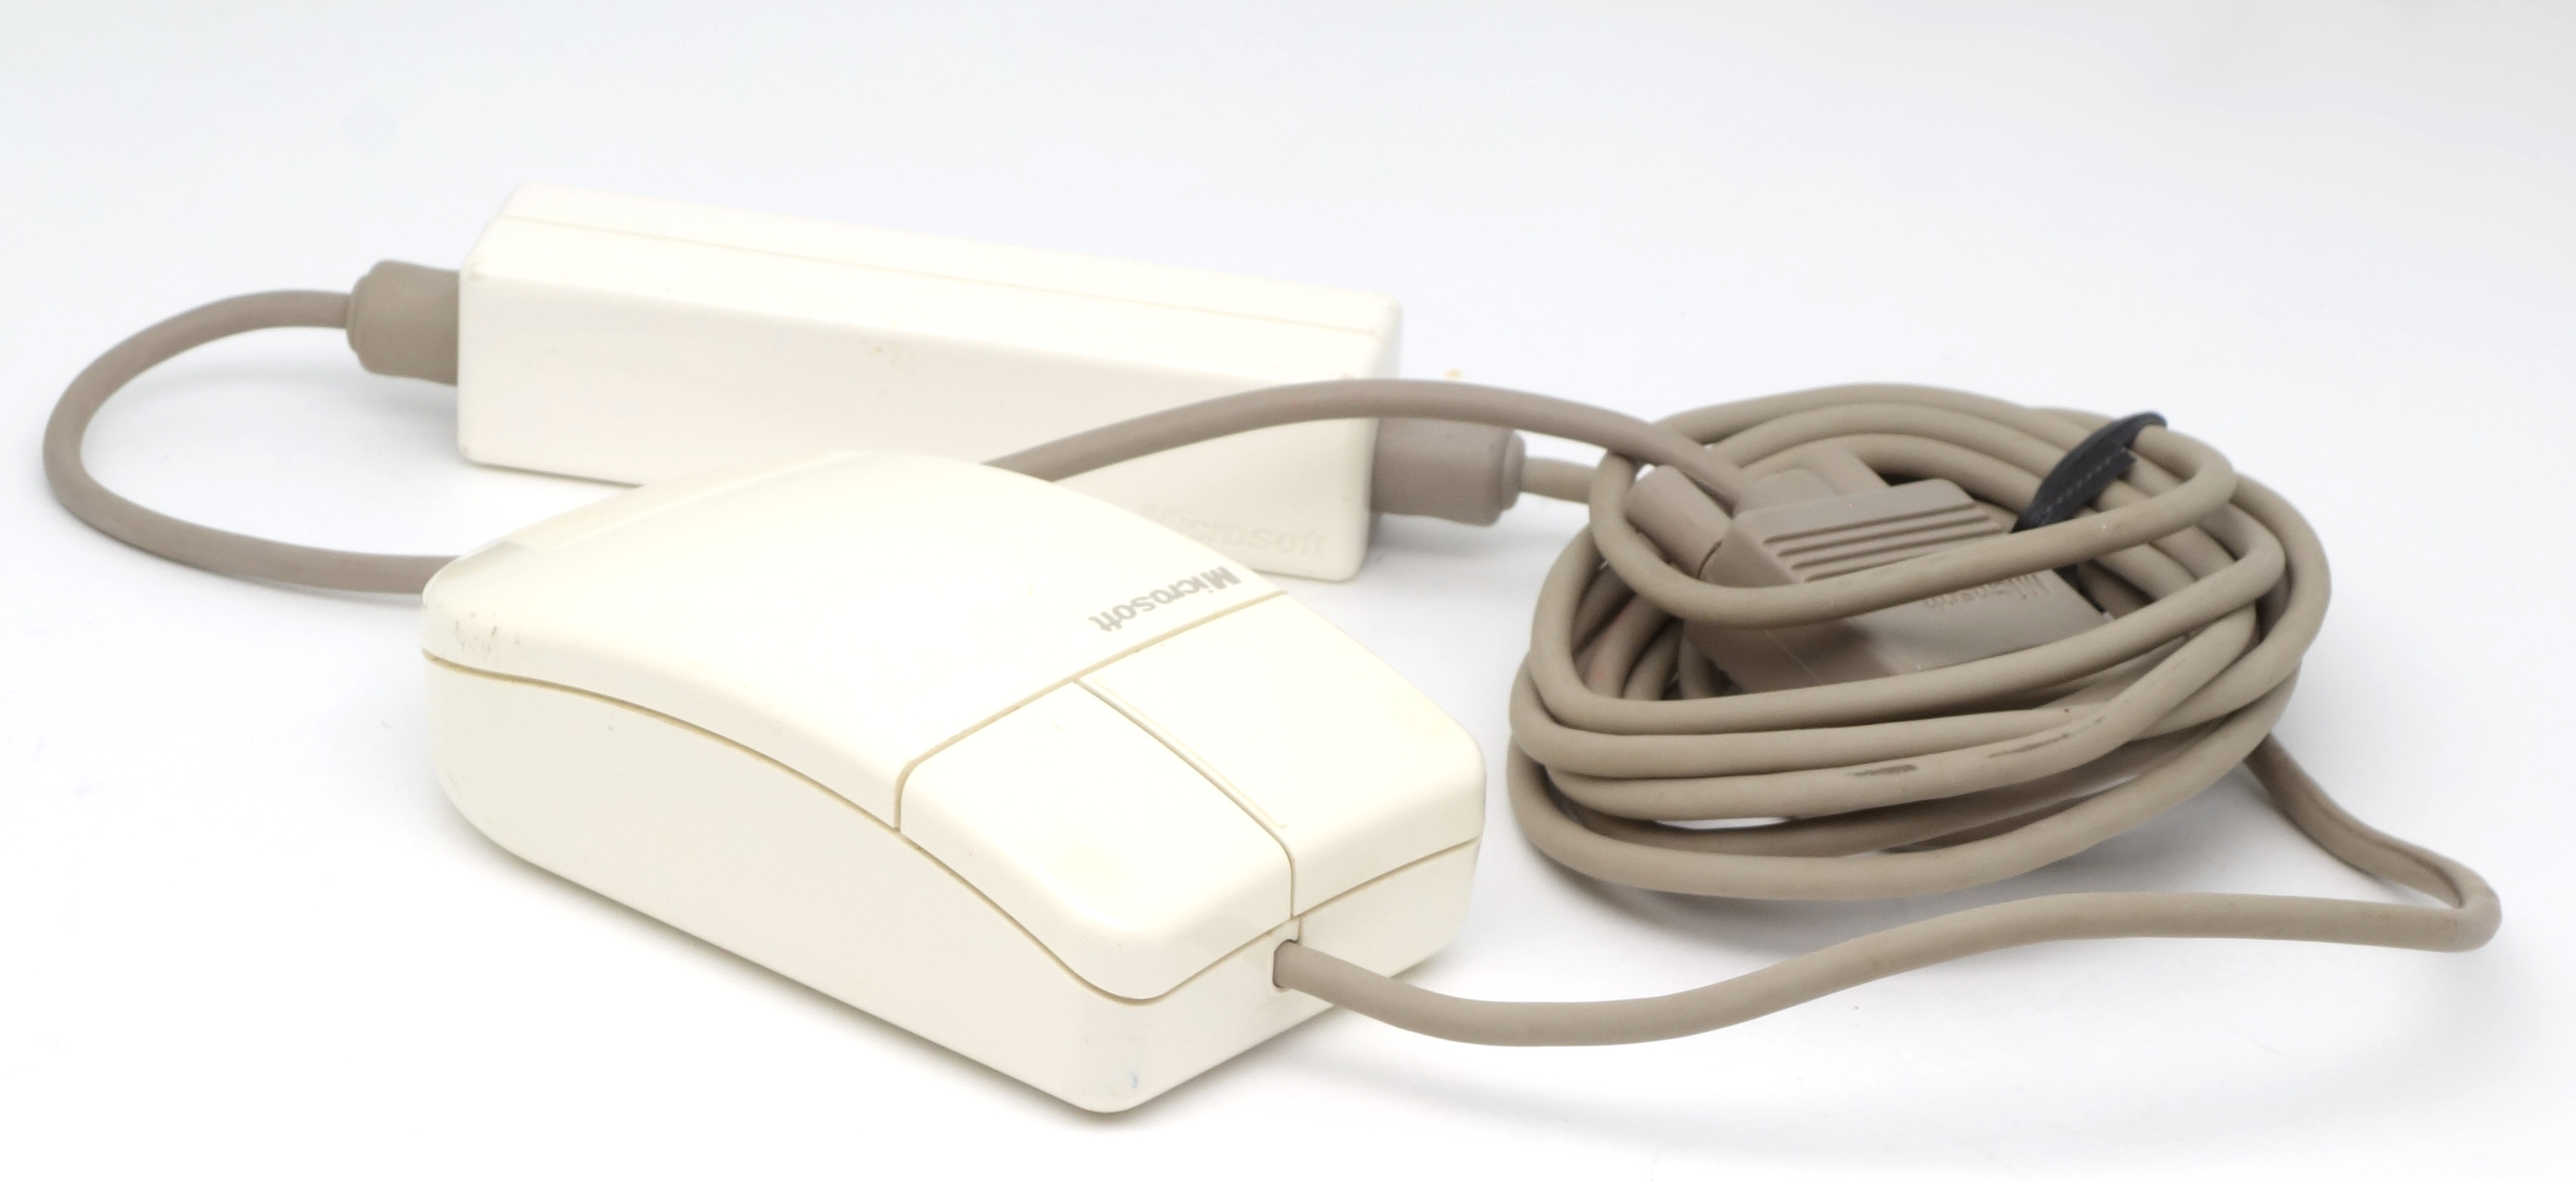
\includegraphics[scale=0.55]{1987_microsoft_dove_bar_mouse/pic_30.jpg}
    \caption{Microsoft Dove Bar Mouse}
    \label{fig:MicrosoftDoveBarPic}
\end{figure}

Beside the new approach for the body shape, third generation had received a bunch of other significant improvements, as in aesthetics and ergonomics, so in technical design. The mouse has a milky-white glossy case (fig. \ref{fig:MicrosoftDoveBarTopAndBottom}); the buttons are significantly larger in size compared to the previous generation, they occupy the front third of the case and are completely integrated into its shape. On the bottom of the case there are low-friction pads, a label with technical data, and a locking ring that can be pushed backward to remove the ball for cleaning.

\begin{figure}[h]
    \centering
    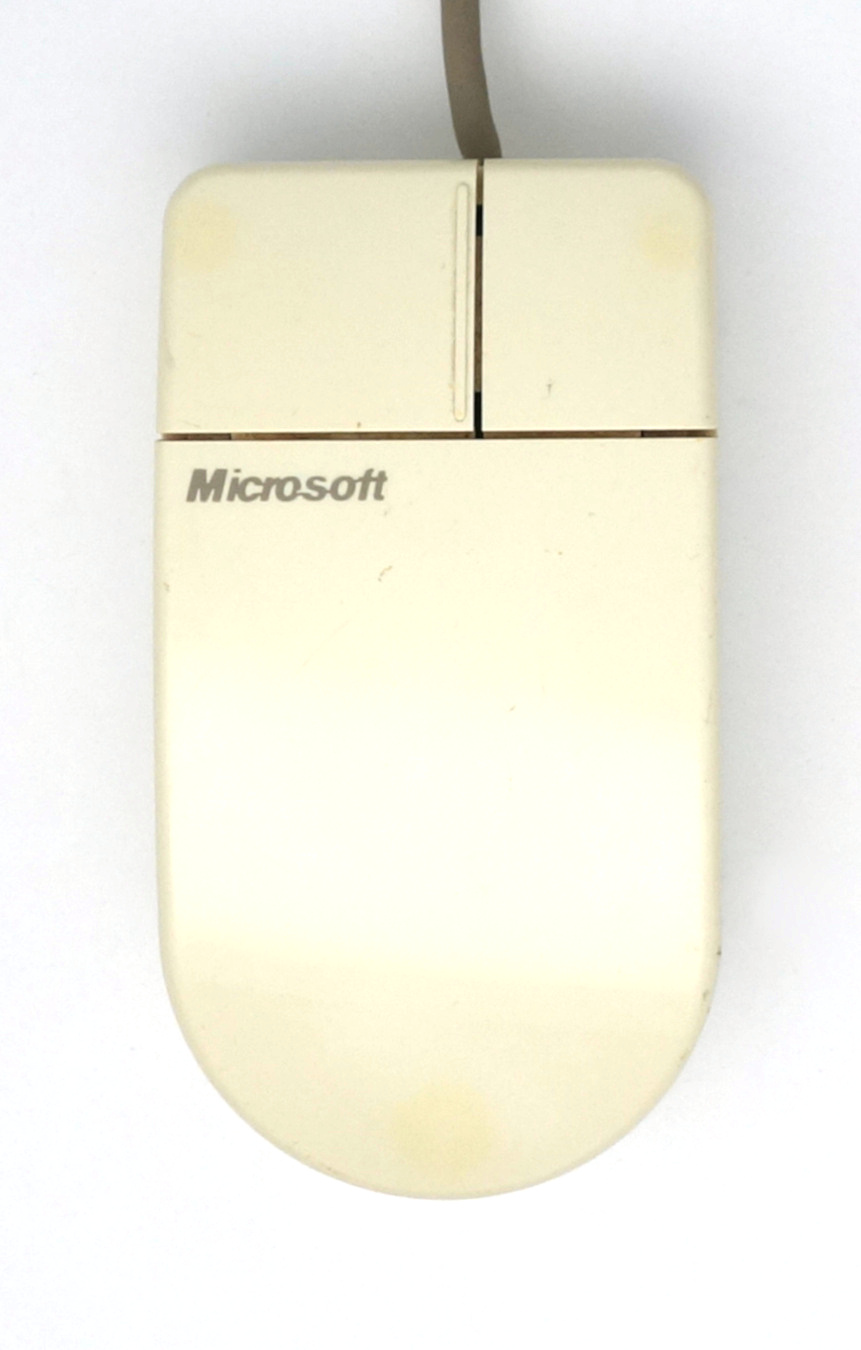
\includegraphics[scale=0.5]{1987_microsoft_dove_bar_mouse/top_30.jpg}
    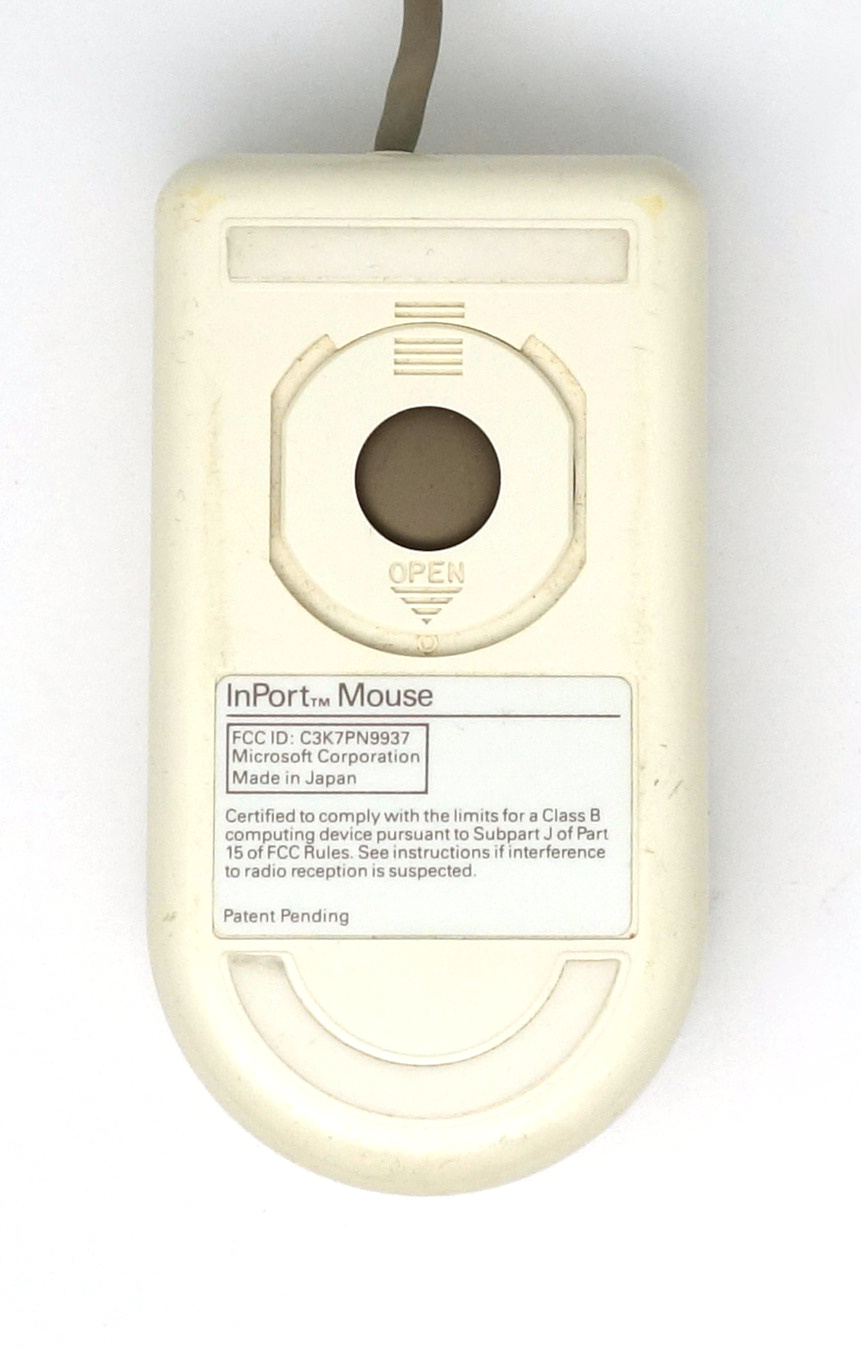
\includegraphics[scale=0.5]{1987_microsoft_dove_bar_mouse/bottom_30.jpg}
    \caption{Microsoft Dove Bar Mouse, top and bottom views}
    \label{fig:MicrosoftDoveBarTopAndBottom}
\end{figure}

The ball is placed in the front part of the mouse, practically in the area where the user's fingers are located. This modification should have noticeably improved the accuracy of cursor positioning compared to mice of previous generations \cite{atkinson}, and apparently the improvement did take place -- at least compared to earlier ALPS  designs, where the ball was located at the edge of the case closest to the user to leave more space for the printed circuit board and buttons. The size of the mouse is typical for the 80s, and is determined not least by the dimensions of the used ALPS unit (fig. \ref{fig:MicrosoftDoveBarSize}). 

\begin{figure}[h]
    \centering
    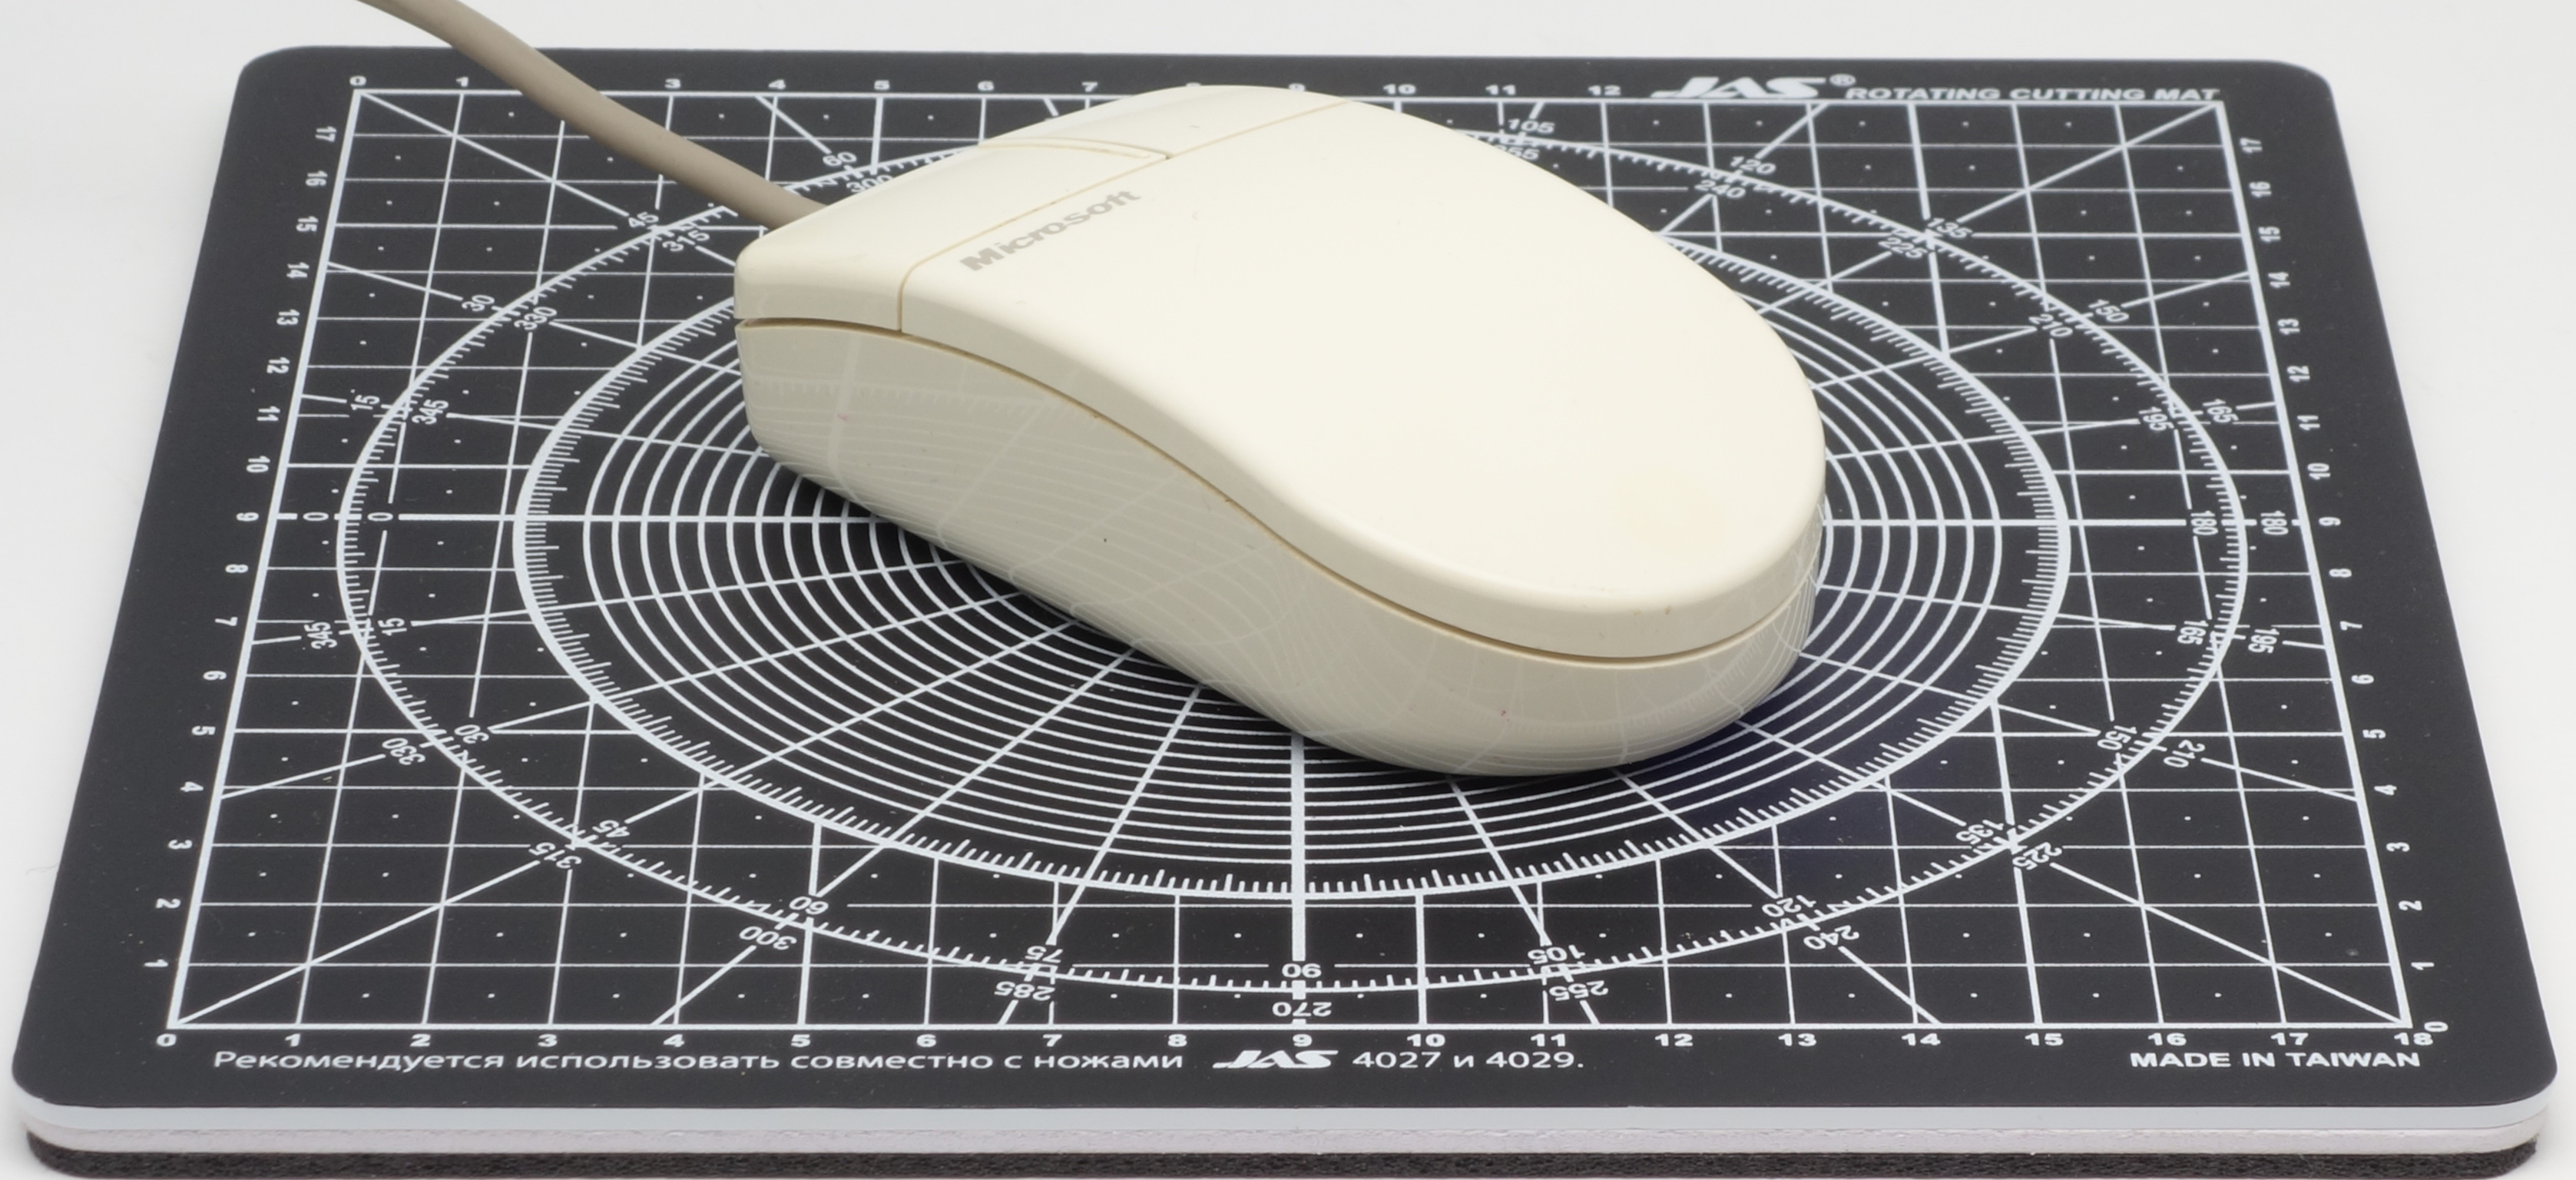
\includegraphics[scale=0.5]{1987_microsoft_dove_bar_mouse/size.jpg}
    \caption{Microsoft Dove Bar Mouse on a graduated pad with a grid step of 1~cm}
    \label{fig:MicrosoftDoveBarSize}
\end{figure}

The Dove Bar Mouse body is symmetrical, with the exception of the buttons, which have different sizes. In addition to the fact that the shape of the sanding block ensures a fairly comfortable hand position (fig. \ref{fig:MicrosoftDoveBarHand}), the comfortable position of the fingers on the buttons  (a very large main button and a smaller, but still quite large, right button) is also worth to note. Previously, other companies tried to use buttons completely integrated into the shape of the body: Logitech did this with the mouse released for Hewlett Packard in 1984, and so did Atari for the mouse of its own computers released in 1985. However, before the Dove Bar Mouse, such a solution was rather an exception to the rule, and the buttons always had the same size: apparently, mouse manufacturers of the 80s were afraid that the user would not be able to reliably determine the boundary between them without looking at the mouse. Microsoft was also concerned about this, so the left button has a small ridge on its right edge so that users could feel the boundary between the buttons. Also, the membrane switches that were used for the buttons in previous Microsoft models were replaced in this one with micro switches in order to minimize the pressing force due to their shorter stroke and better response \cite{doveBarDesign2, doveBarMousePcMag3}.

\begin{figure}[h]
    \centering
    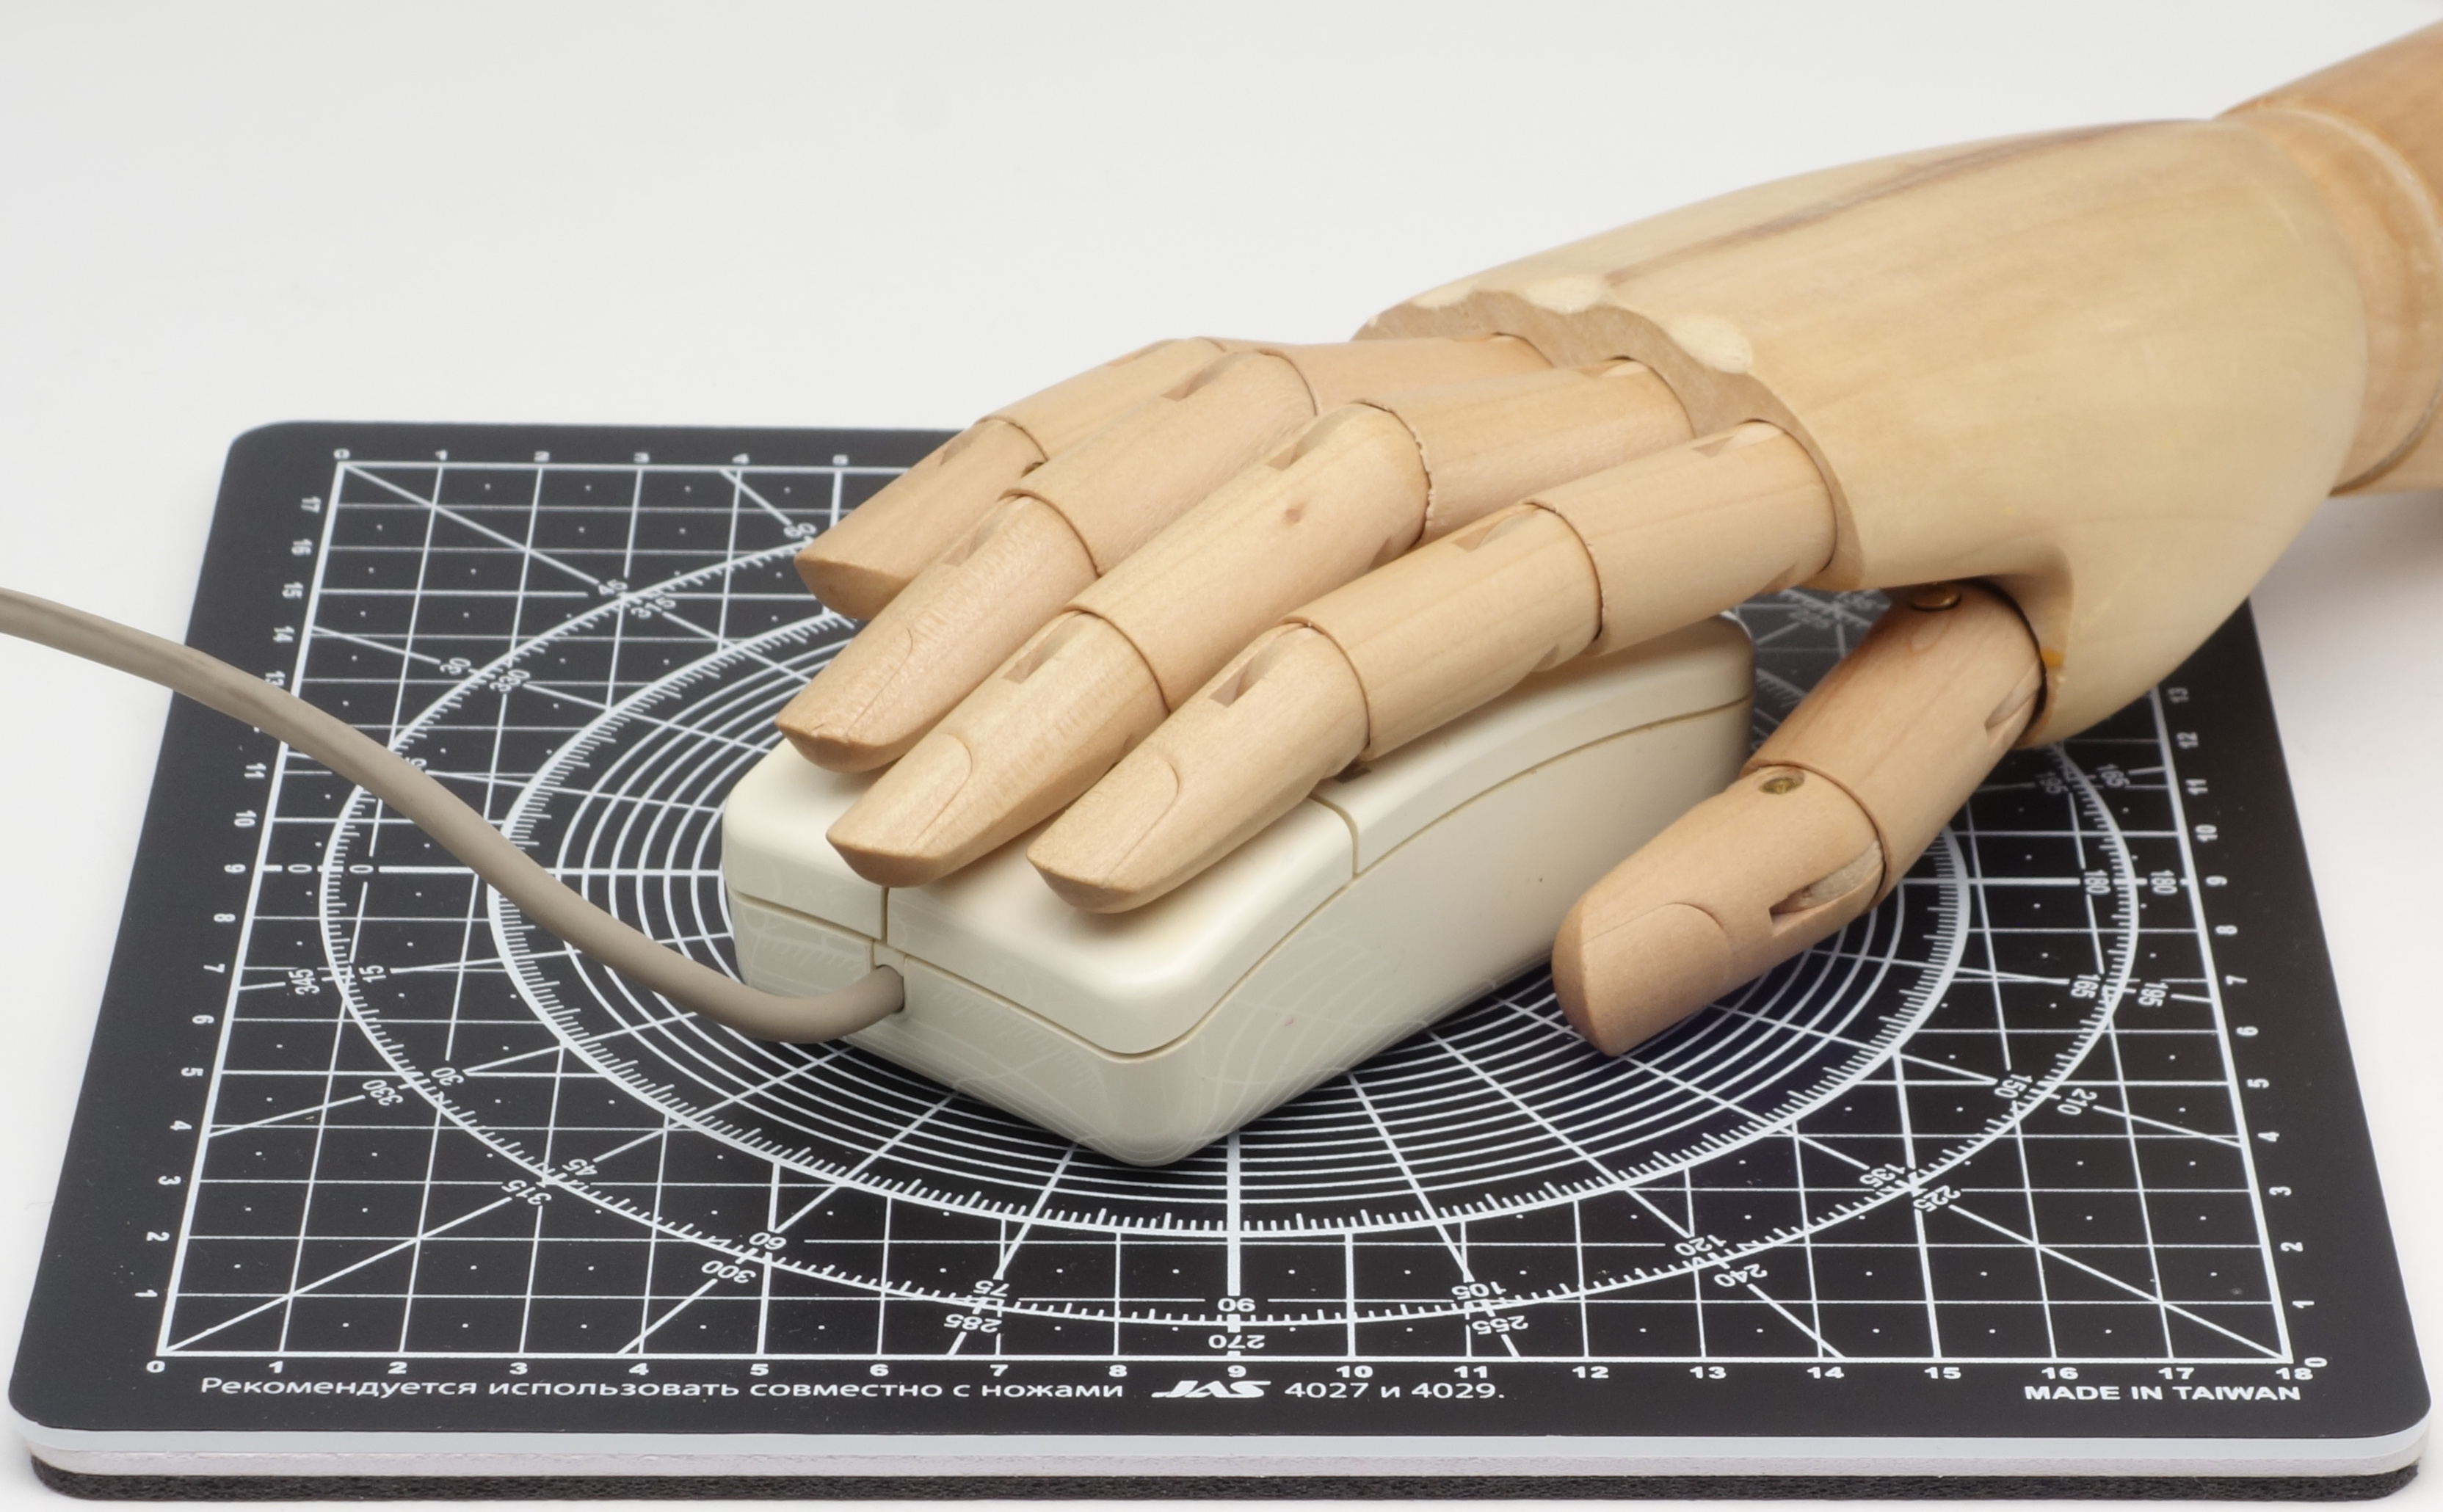
\includegraphics[scale=0.5]{1987_microsoft_dove_bar_mouse/hand.jpg}
    \caption{Microsoft Dove Bar Mouse with a human hand model}
    \label{fig:MicrosoftDoveBarHand}
\end{figure}

The mouse was released in the following modifications: InPort Mouse with a bus interface (Microsoft’s attempt to standardize the interface for connecting quadrature mice, the corresponding adapters and converters for them), and Serial Mouse with a connection to a COM port. In addition to connecting to a special adapter board mounted in the system unit, an external converter shaped as an elongated parallelepiped (so-called ``Mouse Interface'') was also released for InPort Mouse, providing it with a COM port connection (fig. \ref{fig:MicrosoftDoveBarPic}). Finally, there is a later version of the mouse with a serial interface, called ``Microsoft Serial -- PS/2 Compatible Mouse'' (the name indicates the included RS-232 -- PS/2 converter) \cite{doveBarDesign2}.

\begin{figure}[h]
    \centering
    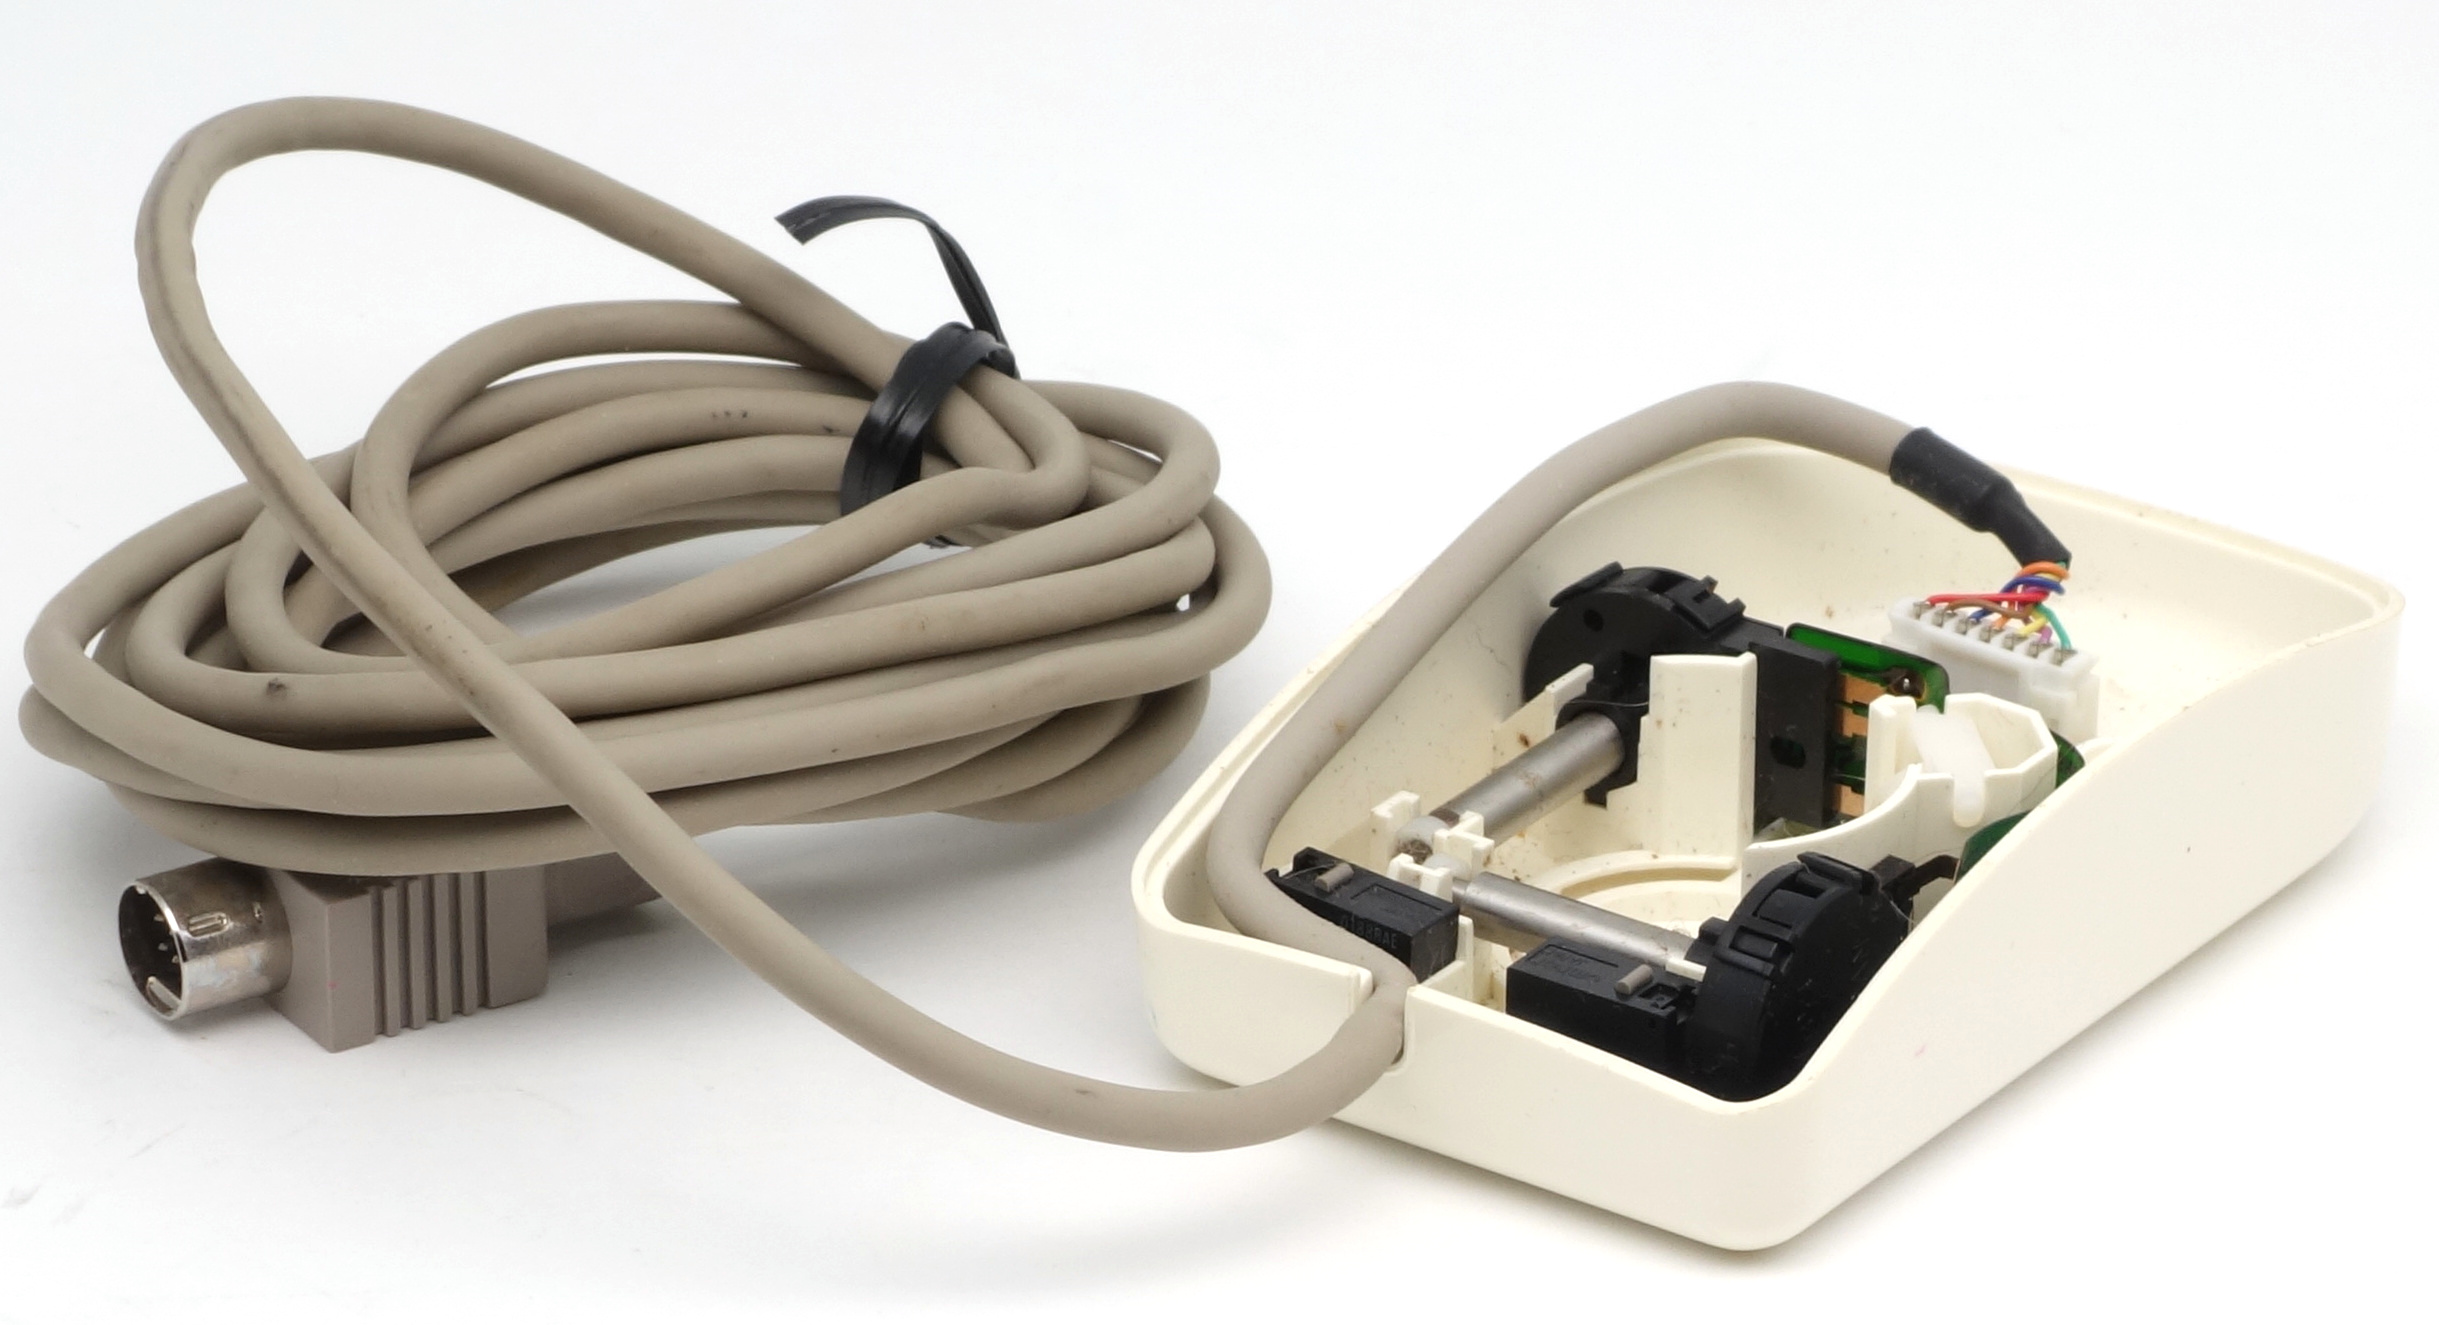
\includegraphics[scale=0.6]{1987_microsoft_dove_bar_mouse/inside1_30.jpg}
    \caption{Microsoft Dove Bar Mouse disassembled}
    \label{fig:MicrosoftDoveBarInside}
\end{figure}

The internal structure of the mouse from 1987 is shown in fig. \ref{fig:MicrosoftDoveBarInside}. Alps usually provided customer companies with solutions based on their standard mouse designs. In particular, this mouse is structurally identical (including the motion conversion unit based on closed mechanical encoders and massive metal rollers with bearings) to the IBM PS/2 mouse, which also appeared on the market in 1987. However, due to the placement of the ball in the front part of the body, the reverse arrangement of components is observed here: the mechanical part is located close to the buttons, which are connected to it and to the printed circuit board by a flexible cable, and the printed circuit board itself is located at the back of the mouse.

\begin{figure}[h]
    \centering
    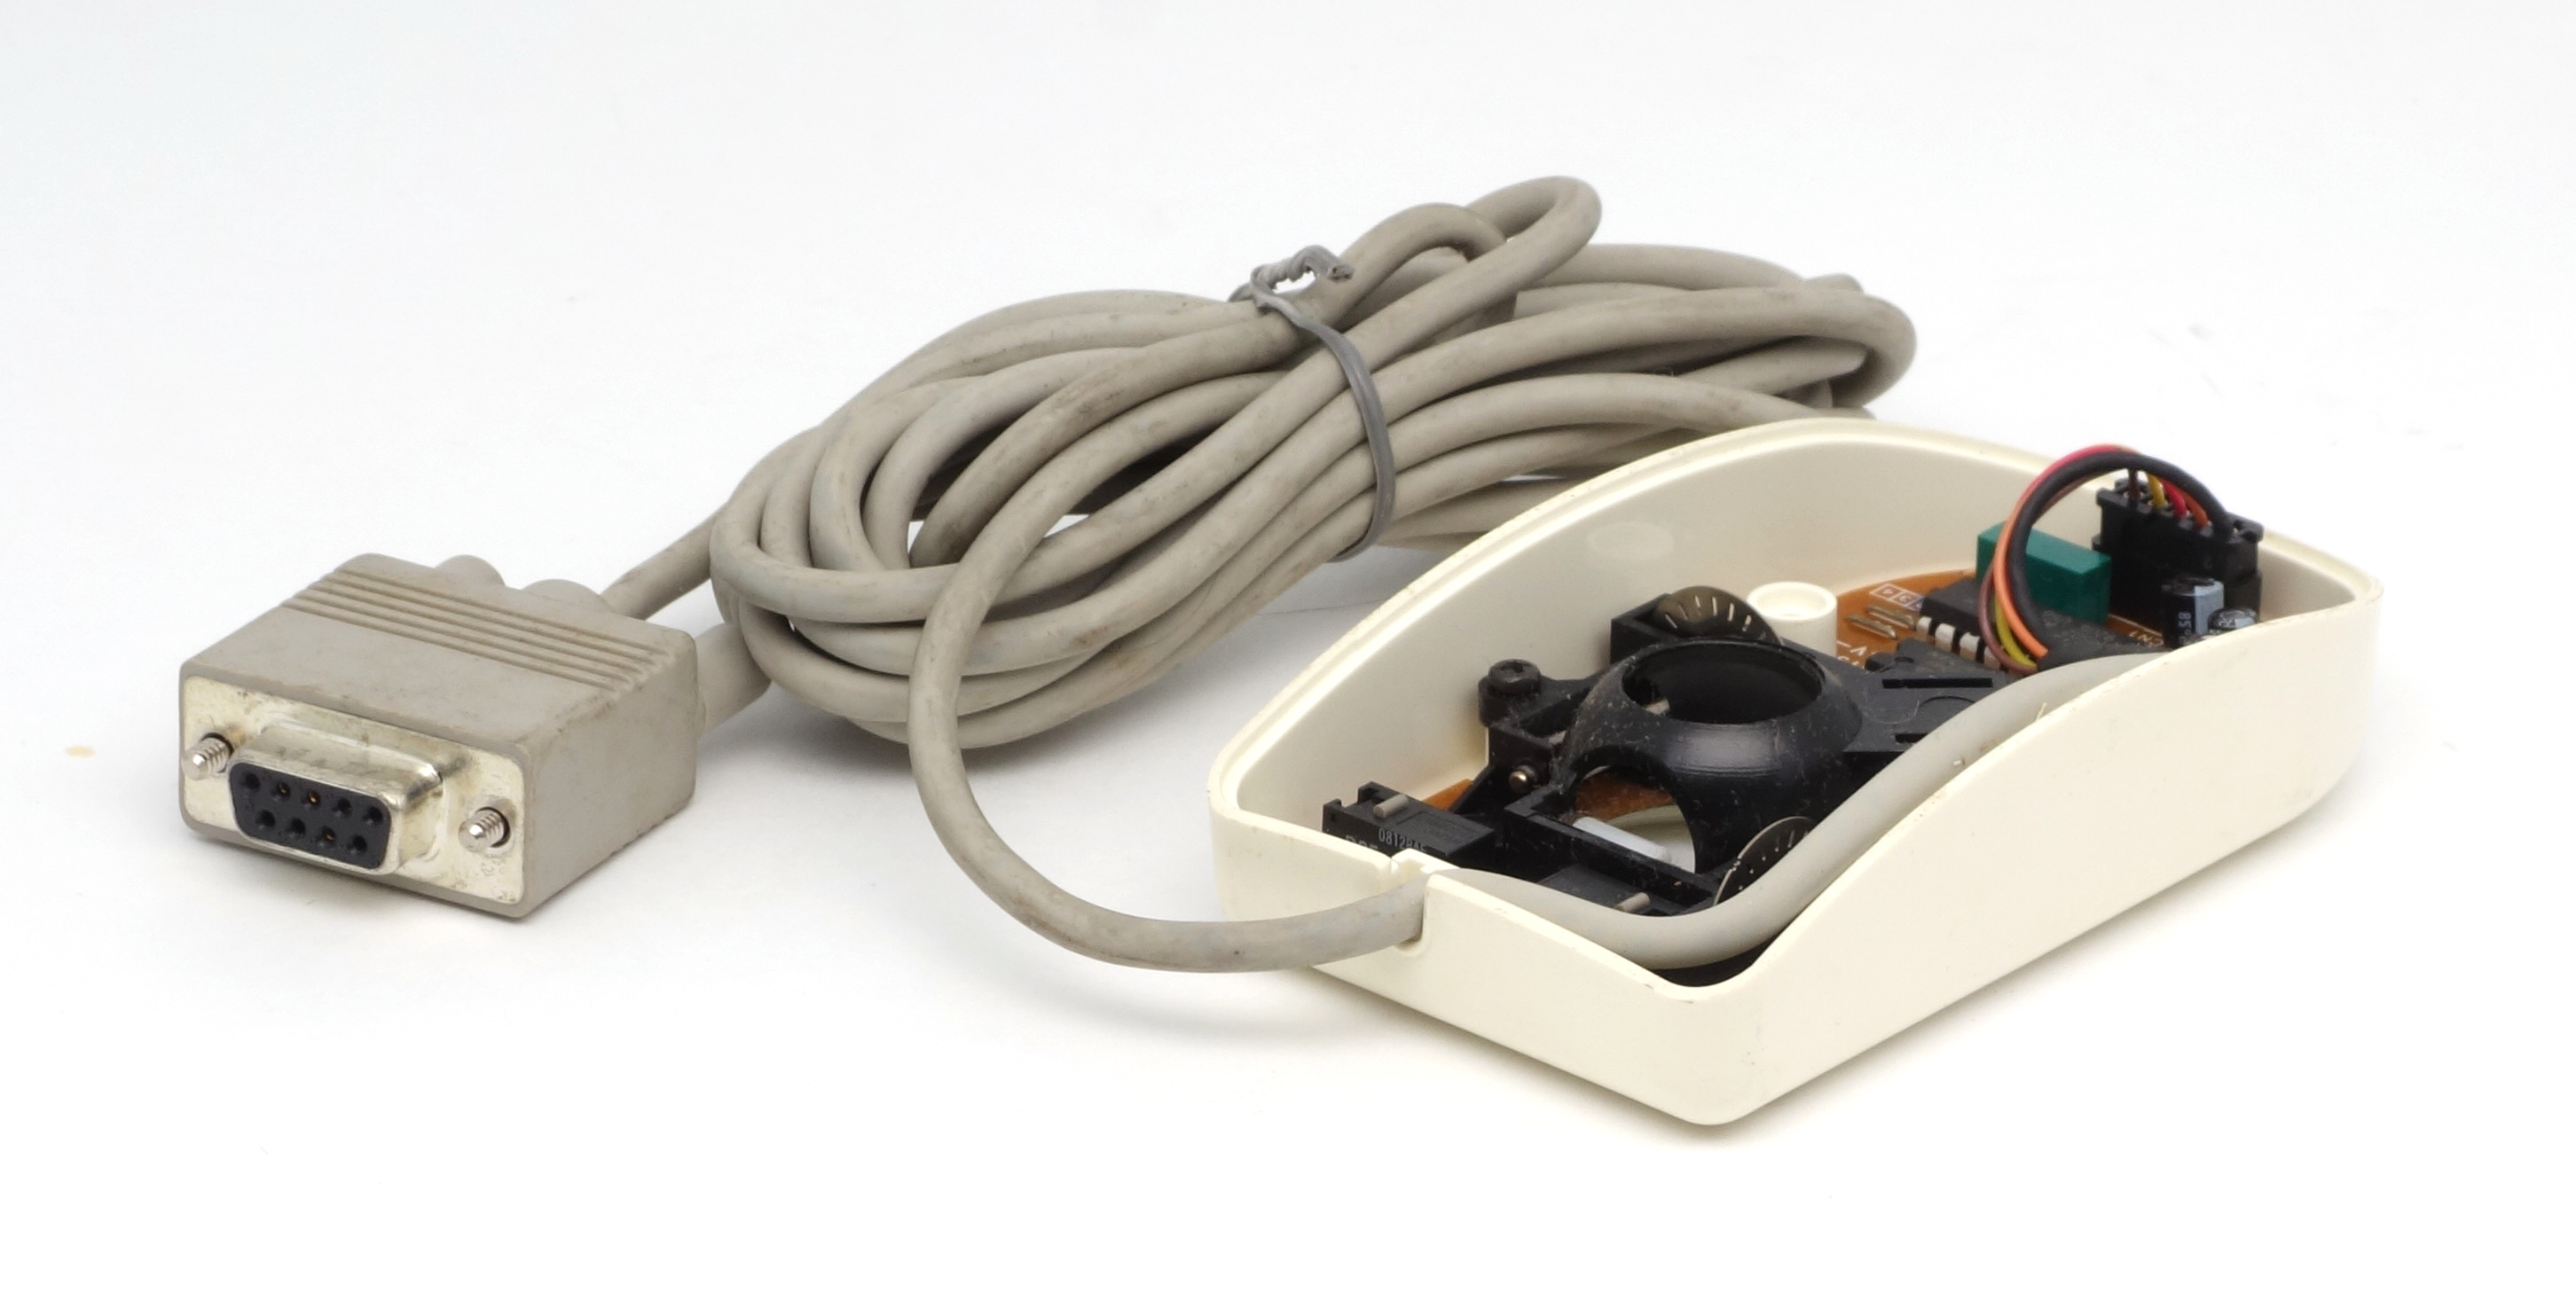
\includegraphics[scale=0.6]{1987_microsoft_dove_bar_mouse/inside2_60.jpg}
    \caption{Microsoft Dove Bar Mouse opto-mechanical version disassembled}
    \label{fig:MicrosoftDoveBarInside}
\end{figure}

Inspired by the success of the new mouse design, in 1991 Microsoft released a mouse in an identical case but with an updated internal design (fig. \ref{fig:MicrosoftDoveBarInside2}), advertised as the ``Contour Microsoft mouse''. This version of the Dove Bar Mouse was no longer manufactured by ALPS, but by Mitsumi. The mouse had used a more contemporary optomechanical motion detection method with a fairly economical mechanical design based on plastic rollers, as well as the noticeable shiny metal disk of the optical interrupter (introduced by Depraz, and also found in early Mitsumi mice), which, according to advertising materials, provided a resolution of 400 dpi \cite{doveBarMouseOldMouses}.

\begin{thebibliography}{9}
\bibitem{doveBarDesign1} Why Microsoft Resurrected A 15-Years-Old Mouse -- Fast Company. \url{https://www.fastcompany.com/90151927/why-we-still-love-using-mice#:~:text=By%20the%20time,the%20soap}
\bibitem{atkinson} Atkinson P. The best laid schemes o’ mice and men : the evolution of the computer mouse // Design and Evolution : Proceedings of Design History Society Conference 2006. Delft, Netherlands, Delft University of Technology, p. 1-20. \url{https://shura.shu.ac.uk/8659/}
\bibitem{doveBarMousePcMag1} The new Microsoft Mouse // PC Magazine, v. 7, No. 2, January, 1988, p. 310--311. \url{https://archive.org/details/PC-Mag-1988-01-26/page/n303/mode/2up}
\bibitem{doveBarMousePcMag2} Stanton T. Microsoft Mouse // PC Magazine, v. 8, No. 3, February 1989, p. 258. \url{https://archive.org/details/PC-Mag-1989-02-14/page/n257/mode/2up}
\bibitem{doveBarMousePcMag3} Stanton T. Microsoft Bus Mouse and Microsoft Serial Mouse // PC Magazine, v. 7, No. 3, February 1988, p. 211--217. \url{https://archive.org/details/PC-Mag-1988-02-16/page/n209/mode/2up}
\bibitem{doveBarDesign2} Microsoft Mouse (3rd gen) - Deskthority wiki. \url{https://deskthority.net/wiki/Microsoft_mouse_(3rd_gen)}
\bibitem{doveBarMouseOldMouses} Microsoft "Dove Bar" Mouse  -- oldmouse.com \url{https://web.archive.org/web/20210417224625/http://oldmouse.com/mouse/microsoft/dovebar.shtml}
\end{thebibliography}
\end{document}
